% verwandte Arbeiten
Bisher wurde kein vollautomatisertes System zur geometrischen Überprüfung der Stentstruktur konzipiert. In diesem Kapitel wird an erster Stelle die Forschung im Bereich der bildbasierten Analyse von Geflechten vorgestellt. Darauffolgend wird auf den aktuellen Stand der automatisierten Inspektion von Stents eingegangen, welche größtenteils auf Verfahren der Bildverarbeitung basiert. Im Anschluss wird auf das Projekt Stents4Tomorrow \cite{flechtmaschine} eingegangen und der bisherige Fortschritt erläutert.


% Bildbasierte Analyse von Geflechten
\section{Bildbasierte Analyse von Geflechten}
Die bildbasierte Analyse von Geflechten wurde bereits von mehrfachen Studien untersucht, was zu diversen Lösungsansätzen geführt hat. So basieren die von Phoenix \cite{phoenix1978mechanical}, Zhang et al. \cite{zhang1999analysis} und Guyader et al. \cite{guyader2013analysis} entworfenen Systeme auf geometrische Beziehungen im Geflecht. Die von Alpyildiz \cite{alpyildiz20123d} veröffentlichte Arbeit schlägt dreidimensionale Garnwege im Geflecht vor, welche für die Simulation der Geflechtgeometrie notwendig sind. Darüber hinaus entwickelten Hunt et al. \cite{hunt2019machine} ein Computer-Vision-System für die Echtzeitvermessung des Flechtwinkels in der Produktion. Das System verwendet eine 2D diskrete Fourier-Transformation für die Verarbeitung der Bilder und erzielt eine Genauigkeit von $\pm$1-2 Grad bei der Vermessung von einzelnen Winkeln. \cite{hunt2019machine} Liu et al. \cite{liu2019automatic} implementierten ein ähnliches System unter der Verwendung des Canny-Algorithmus \cite{canny1986computational} und der Hough-Transformation \cite{duda1972use}.

\mypar Xiao et al. untersuchten die Vermessung der Picklänge und des Flechtwinkels mit unterschiedlichen Ansätzen in mehreren Studien. Beim ersten Ansatz \cite{xiao2018measurement} wurden vielfältige Kantendetektoren eingesetzt, um die Ecken im Bild zu ermitteln. Diese Herangehensweise wurde darauffolgend in \cite{xiao2019surface} durch die Einführung des ''local edge extreme''-Algorithmus ersetzt. In einer weiteren Veröffentlichung \cite{pei2019surface} wurde für die Vermessung der oben genannten Größen eine auf die sogenannte ''gray projection'' basierte Methode eingeführt, mit der eine hohe Genauigkeit erzielt wurde. Darüber hinaus wurde ein Faster R-CNN-Modell in \cite{xiao2020surface} trainiert, um Picklängen und Flechtwinkel in Bildern, wie in Abbildung \ref{fig:faster_rcnn} aufgezeigt, zu lokalisieren und messen.

\begin{figure}[h!]
\centering
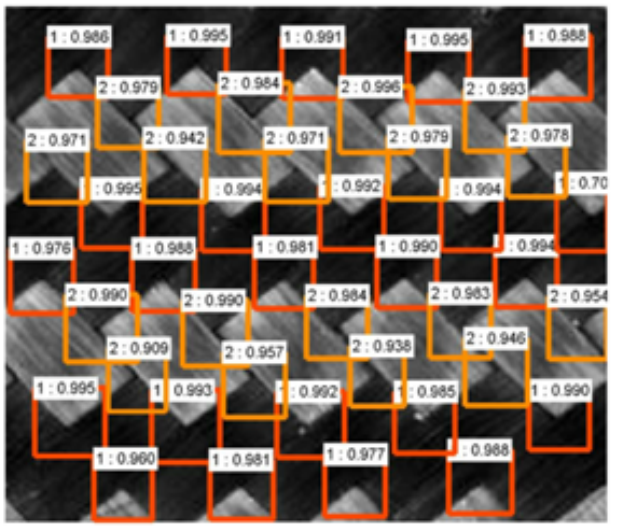
\includegraphics[width=7cm]{98_images/xiao_2020.png}
\caption{Testergebnisse der Anwendung eines Faster R-CNN auf Bilder von Geflechten. Entnommen aus \cite{xiao2020surface}.}
\label{fig:faster_rcnn}
\end{figure}


% Visuelle Inspektion von Stents
\section{Visuelle Inspektion von Stents}
Es wurden bereits einige Untersuchungen und Studien im Bereich der visuellen Inspektion von Stents durchgeführt. Eine von Farmer \cite{farmer2005automated} durchgeführte Studie führte ein Bildverarbeitungssystem ein, um die Drähte und Kanten des Stents zu untersuchen. Das System wird von zwei Sensorenpaketen betrieben. Das erste Paket wird für die Überprüfung der Drähte und Kanten verwendet, wohingegen das zweite Paket die Fläche zwischen den Drähten betrachtet. Das entworfene System verfehlte 0,08{\%} der Defekte, identifizierte 8{\%} der Defekte falsch positiv und konnte mit einer Geschwindigkeit von 18 mm pro Minute und sechs Sekunden betrieben werden. \cite{farmer2005automated}

\mypar In der von Ibraheem und Binder \cite{ibraheem2009automated} veröffentlichten Arbeit, wird eine Zeilenkamera verwendet, um ein hochauflösendes Bild des gesamten Stents aufzunehmen. Zur Erkennung von Fehlern werden unterschiedliche Verfahren aus der Kantendetektion und Bildsegmentierung angewendet. Somit werden bogenförmige Segmente an den Kreisbögen des Stents im Bild angepasst. Anhand dieser Anpassung können die Mittelpunkte und Radien der Bögen bestimmt werden. Aus den Abweichungen zwischen den Werten können lokale Fehler detektiert werden. \cite{ibraheem2009automated}

\begin{figure}[h!]
\centering
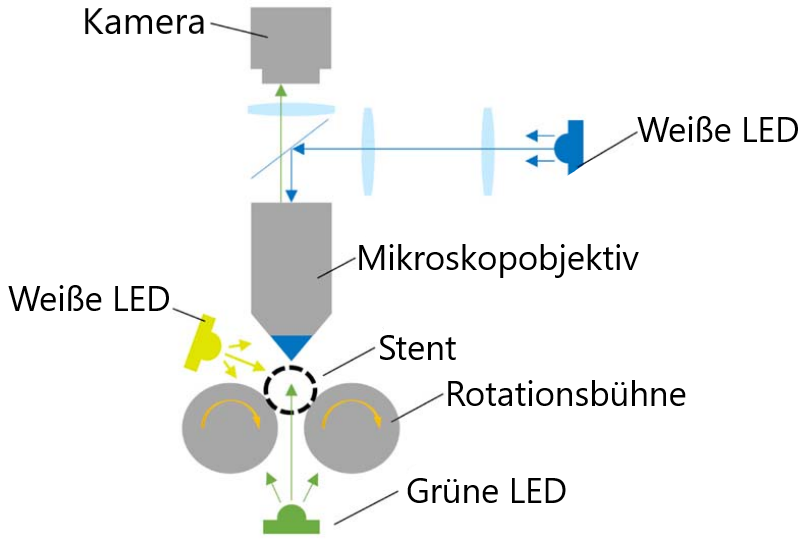
\includegraphics[width=7cm]{98_images/aufbau_bermudez.png}
\caption{Aufbau des von Bermudez et al. 2016 entworfenen Systems mit einem dreifachen Beleuchtungssystem. Entnommen und übersetzt aus \cite{bermudez2017stent}.}
\label{fig:bermudez_aufbau}
\end{figure}

\mypar In einer von Bermudez et al. \cite{bermudez2017stent} durchgeführten Studie werden Bilder, wie in Abbildung \ref{fig:bermudez_aufbau} zu sehen, mithilfe einer Mikroskopanordnung, einem dreifachen Beleuchtungssystem und einer Rotationsbühne aufgenommen. Anhand einer Segmentierung kann der Draht des Stents vom Hintergrund des Bildes isoliert werden (siehe Abbildung \ref{fig:bermudez_stent_mask}). Durch die Anwendung morphologischer Operatoren wird das segmentierte Bild weiterverarbeitet, um Kanten sichtbar zu machen. Im Anschluss werden die Drahtbreite und Kantenrundheit auf geometrische Fehler untersucht \cite{bermudez2017stent}. Eine weitere Veröffentlichung stellte ein verbessertes System mit einem verbesserten Vermessungssystem vor. Hierfür werden sogenannte Confocal und Coherence Scanning Interferometry (kurz CSI \cite{de2011coherence}) angewendet, um die Form, Textur und Defekte der Oberfläche von Stents anhand von 3D-Messtechnik evaluieren zu können \cite{bermudez2017optical}. Des Weiteren wird in einer darauffolgenden Studie ein Klassifikator eingeführt, welcher Defekte von Stents an der Oberfläche oder Kanten in unterschiedliche Arten einstufen kann \cite{bermudez2017automated}.

\begin{figure}[h!]
\centering
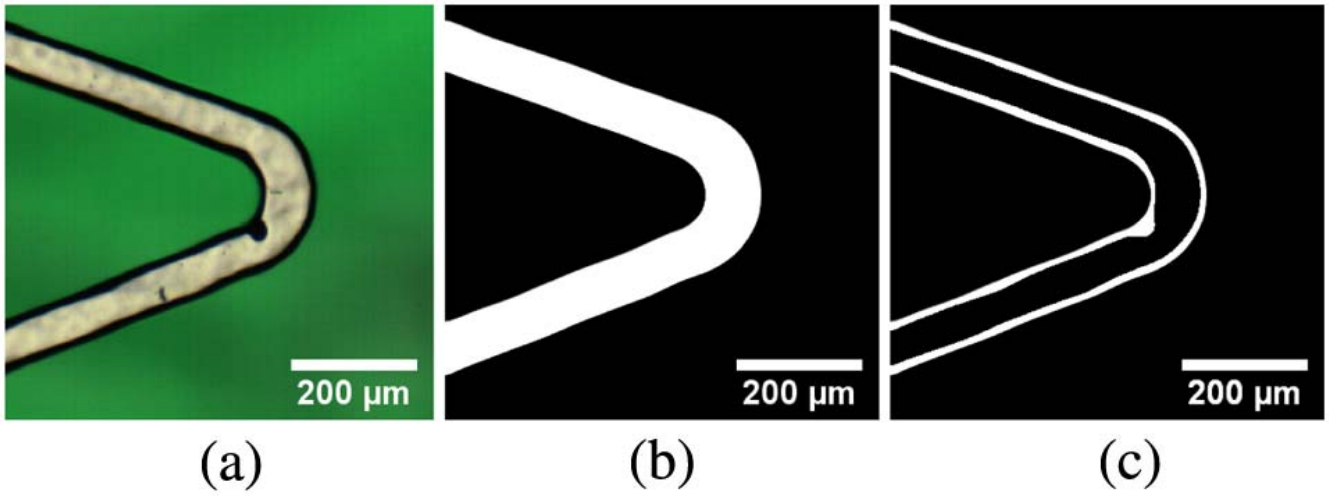
\includegraphics[width=10cm]{98_images/stent_edge_mask.png}
\caption{Stent mit einem Rissdefekt: (a) ursprüngliches Bild, (b) Maske der Oberfläche, (c) Maske der Kanten. Entnommen aus \cite{bermudez2017stent}.}
\label{fig:bermudez_stent_mask}
\end{figure}


% Stents4Tomorrow
\section{Stents4Tomorrow}
Im Rahmen des Stents4Tomorrow-Projekts \cite{flechtmaschine} soll der Prozess der visuellen Inspektion von Stents während der Produktion automatisieren. Ein wichtiger Bestandteil ist die Erkennung von Fehlern im Geflecht. Houssem \cite{houssem} setzte sich sowohl mit der Berechnung des Flechtwinkels als auch mit der Erkennung von Unregelmäßigkeiten im Flechtmuster auseinander. Ähnlich wie in \cite{hunt2019machine} wurden die Hough- und 2D diskrete Fourier-Transformation angewendet und miteinander verglichen. Hierbei führte die zweidimensionale diskrete Fourier-Transformation zu besseren Ergebnissen bei Bildern aller Flechtwinkel. Zur Überprüfung des Flechtmusters wurde die U-Net-Architektur implementiert und mit einem Convolutional Autoencoder verglichen. U-Net zeigte eine höhere Leistung vor. \cite{houssem}

\mypar Zusammen mit dem Flechtwinkel ist die Picklänge ein wichtiger Bestandteil der Geometrie von Stents. Aus diesem Grund untersuchte Schorle \cite{felix} die Vermessung der Picklänge anhand unterschiedlicher Methoden. Durch die Anwendung faltender neuronaler Netze konnte eine Genauigkeit von 0,267 Millimetern bei der Vermessung der durchschnittlichen Länge von Picks auf einer Linie erreicht werden. \cite{felix}

\mypar Neben der zuverlässigen Fehlererkennung im Stent ist die Effizienz des Systems bei der Korrektur der erkannten Fehler wichtig. Djamal \cite{aulia} setzte sich mit der Optimierung dieses Vorgangs auseinander. Somit wurden sechs Abläufe zur Fehlerkorrektur entworfen. Bei den zwei nicht-optimierten Vorgängen wurden zwei optimale Ansätze gefunden. Zudem konnte eine optimale Lösung für die Genauigkeit und für die Ablaufzeit konzipiert werden. \cite{aulia}

\mypar Der Grundbestandteil der Fehlerkorrektur ist das entsprechende System, um diese auszuführen. In \cite{valentin} wird das Konzept eines kamerabasierten Korrektursystems zur Verbesserung des Flechtprozesses von Stents vorgestellt. Die Funktionsweise des Algorithmus des Systems ist hierbei in drei grundlegende Schritte aufgeteilt: Erst wird die Picklänge vermessen, darauffolgend wird über die Korrektur entschieden und im Anschluss wird diese spezifiziert. Das vorgestellte System zeichnet sich durch die Verwendung mehrerer arbeitsteiliger Convolutional Neural Networks aus. Diese sind in einer Programmlogik miteinander verknüpft, sodass Messfehler besser eingegrenzt werden können. \cite{valentin}